\documentclass[t, pdftex, aspectratio=169]{beamer}  % for 16:9 slides
\usetheme{CambridgeUS}
\usecolortheme{crane}

\usepackage{graphicx}
\graphicspath{{../tikz_figures/}}
\DeclareGraphicsExtensions{.pdf,.jpeg,.png, .jpg, .PNG}

\usepackage{tikz}
\usetikzlibrary{arrows}
\usetikzlibrary {arrows.meta}
\usetikzlibrary{intersections}
\usetikzlibrary{calc, quotes}
\usetikzlibrary{external}
\usetikzlibrary{positioning}
\usetikzlibrary{shapes.geometric, shapes.misc}
\usetikzlibrary{tikzmark}
\usetikzlibrary{decorations.pathreplacing}

\title{Triton Dot Operator Lowering for AMD GPU\\Design Review}
\author{Lixun Zhang}
\date{\today}


\begin{document}

\frame{\maketitle}
	
\begin{frame}{Outline}
\tableofcontents
\end{frame}
	
\section{\emph{blockwise\_gemm\_v2} operator lowering in rocMLIR}

\begin{frame}
  \frametitle{Context of blockwise\_gemm\_v2 op}

  \begin{tikzpicture}[overlay, remember picture]
    \coordinate (orig) at (0,.5);
    \draw [fill=cyan] (orig) circle (2pt);

    \node [below right, inner sep=0] at (orig){
      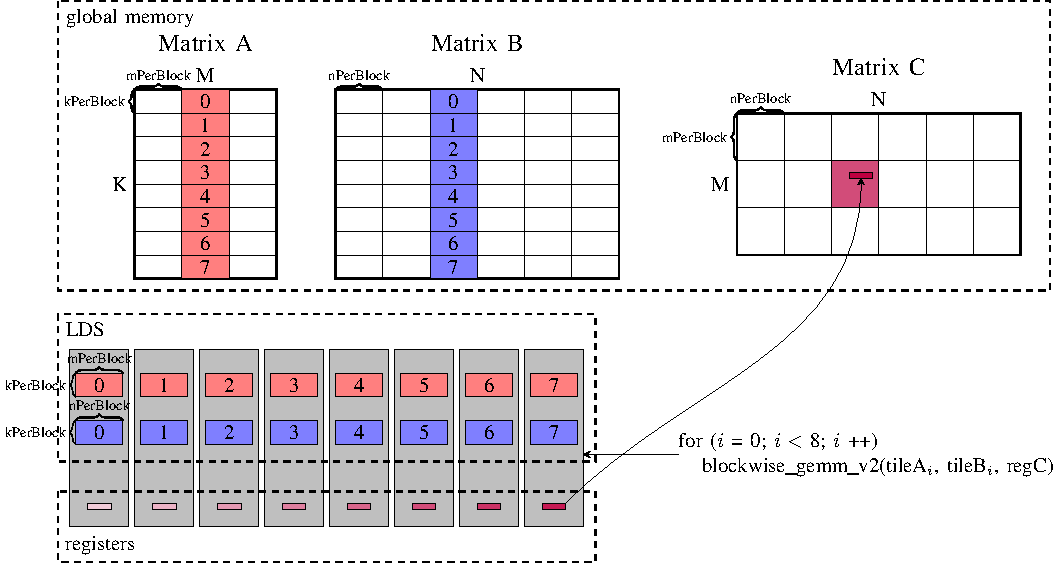
\includegraphics[width=4in]{gridwise_gemm_to_blockwise}};

    \node [below right, align=left] at ($(orig)+(10.3, 0)$) {
      - also tt.dot\\
      - rock.global\_load\\
      - rock.global\_store\\
      - rock.in\_bounds\_load\\
      - rock.in\_bounds\_store\\
      - vector.extractelement\\
      - vector.insertelement\\
      - memref.load
    };
  \end{tikzpicture}
\end{frame}


\begin{frame}
  \frametitle{blockwise\_gemm to xdlops\_gemm}

  \begin{tikzpicture}[overlay, remember picture]
    \coordinate (orig) at (0,.5);
    \draw [fill=cyan] (orig) circle (2pt);

    \node [below right, inner sep=0] at ($(orig)+(0, 1)$){
      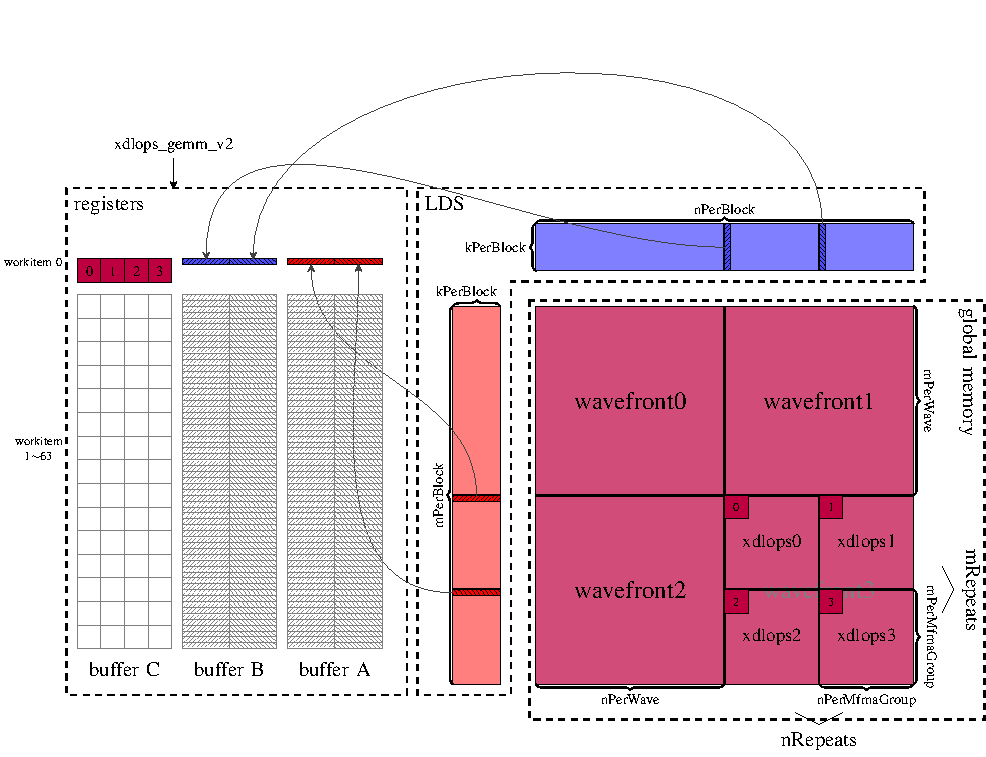
\includegraphics[width=4in]{blockwise_gemm_to_threadwise}};

    \node [below right, align=left] at ($(orig)+(10.3, 0)$) {
      - rock.xdlops\_gemm
    };
  \end{tikzpicture}
\end{frame}


\begin{frame}
  \frametitle{xdlops\_gemm to mfma instructions}

  \begin{tikzpicture}[overlay, remember picture]
    \coordinate (orig) at (0,.5);
    \draw [fill=cyan] (orig) circle (2pt);

    \node [below right, inner sep=0] at ($(orig)+(8, 1.2)$){
      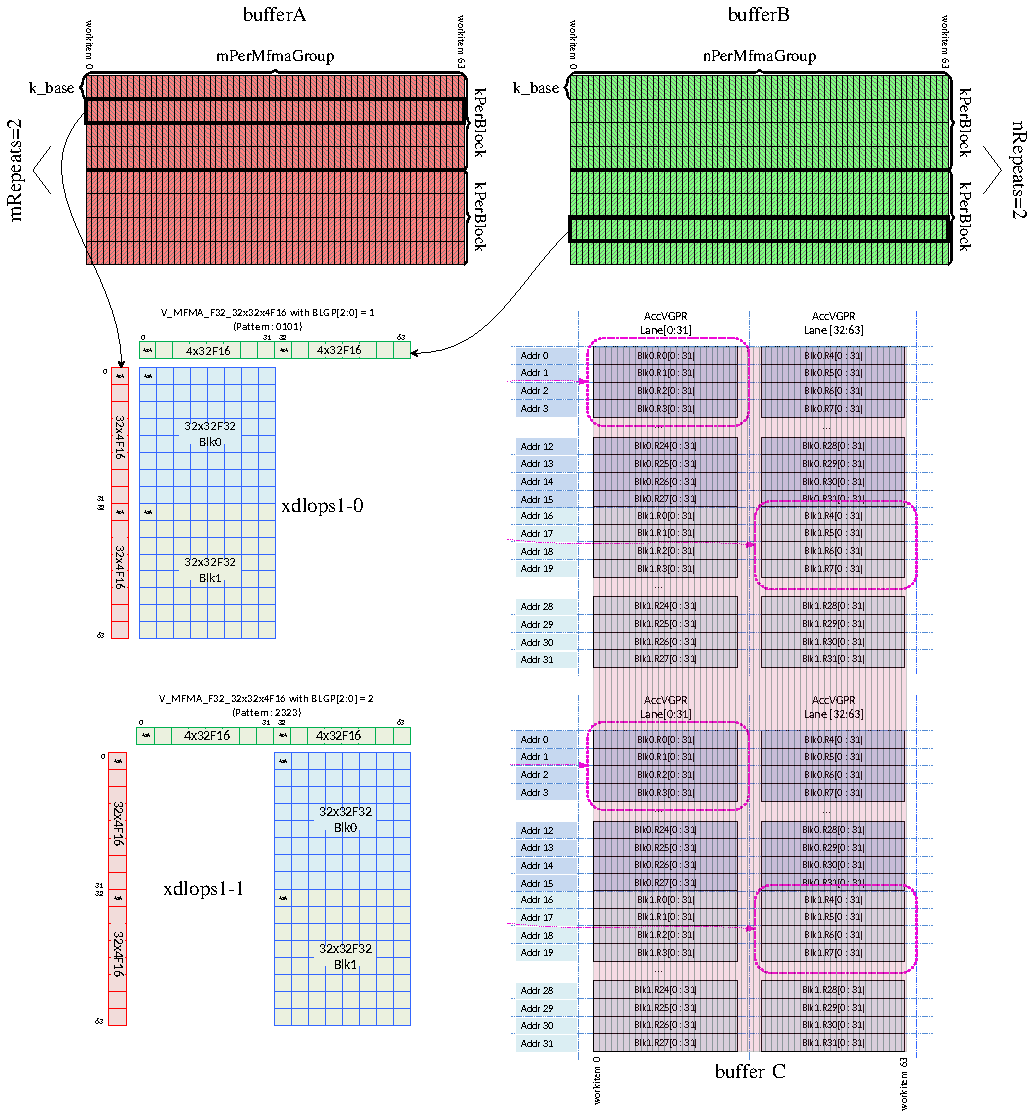
\includegraphics[width=3in]{threadwise_lowering}};

    \node [below right, align=left] at (orig) {
      - amdgpu.mfma\\
      - adafad
    };
  \end{tikzpicture}
  
\end{frame}

\begin{frame}
  \frametitle{Other Lowering Passes}
  \begin{itemize}
  \item sugar-to-loops: amdgpu.raw\_buffer\_load, gpu.warp\_swizzle
  \item rock-to-gpu
    \begin{itemize}
      \item rock::WorkgroupBarrierOp $\rightarrow$  gpu::BarrierOp
      \item rock::LDSBarrierOp $\rightarrow$  amdgpu::LDSBarrierOp
      \item rock::WorkgroupIdOp $\rightarrow$  gpu::BlockIdOp
      \item rock::WorkitemIdOp $\rightarrow$  gpu::ThreadIdOp
      \item func::ReturnOp $\rightarrow$  gpu::ReturnOp
    \end{itemize}
  \end{itemize}
\end{frame}


\section{The Problem}

\begin{frame}
  \frametitle{Work Distribution}
  Since mma (NVIDIA) and mfma (AMD) instructions require special layout of elements in registers, each thread cannot access data in the naive way
  \begin{itemize}
  \item rocMLIR
    \begin{itemize}
    \item We use coordinate transformation to virtually change the data layout in tensor/matrix
    \item Each thread can access elements using their (bid, tid, laneid)
    \end{itemize}
  \item Triton
    \begin{itemize}
    \item Encodings are used to decorate the tensor type to indicate which thread can access which element
    \item convert\_layout pass computes the correct encodings for arguments to tt.dot
    \end{itemize}
  \end{itemize}
\end{frame}
	
\section{TODOs}

\begin{frame}
  \frametitle{TODOs}
  \begin{itemize}
  \item Understanding how encodings are used in triton to distribute work for each thread
  \item Implement (or reuse if possible) encodings for AMD mfma supported layouts
  \item Add vector and memref dialects
  \end{itemize}
\end{frame}
	
\end{document}
%%% Local Variables:
%%% mode: latex
%%% TeX-master: t
%%% End:
